\documentclass[main.tex]{subfiles}
\begin{document}

\section{Постановка задачи}
\begin{enumerate}
\item Составить задачу линейного программирования следующего вида:
	\begin{itemize}
	\item 4 переменные
	\item 2 ограничения в виде равенств
	\item 1 ограничение в виде неравенства со знаком $\geq$ и одно со знаком $\leq$
	\item 1 переменная имеет ограничение на знак.
	\end{itemize}
\item Привести задачу к виду, необходимому для применения симплекс-метода.
\item Построить к данной задаче двойственную и также привести к виду, необходимому для применения симплекс-метода.
\item Решить обе задачи симплекс-методом с выбором начального приближения методом искусственного базиса.
\item Решить обе задачи методом перебора крайних точек.
\item Разработать схему восстановления прямой задачи по решению двойственной.
\end{enumerate}
Алгоритмы, требуемые для решения задачи, реализовать в таком виде, чтобы их можно было использовать в качестве подпрограмм в следующих лабораторных работах.
\section{Исследование применимости метода}
\section{Описание алгоритмов}
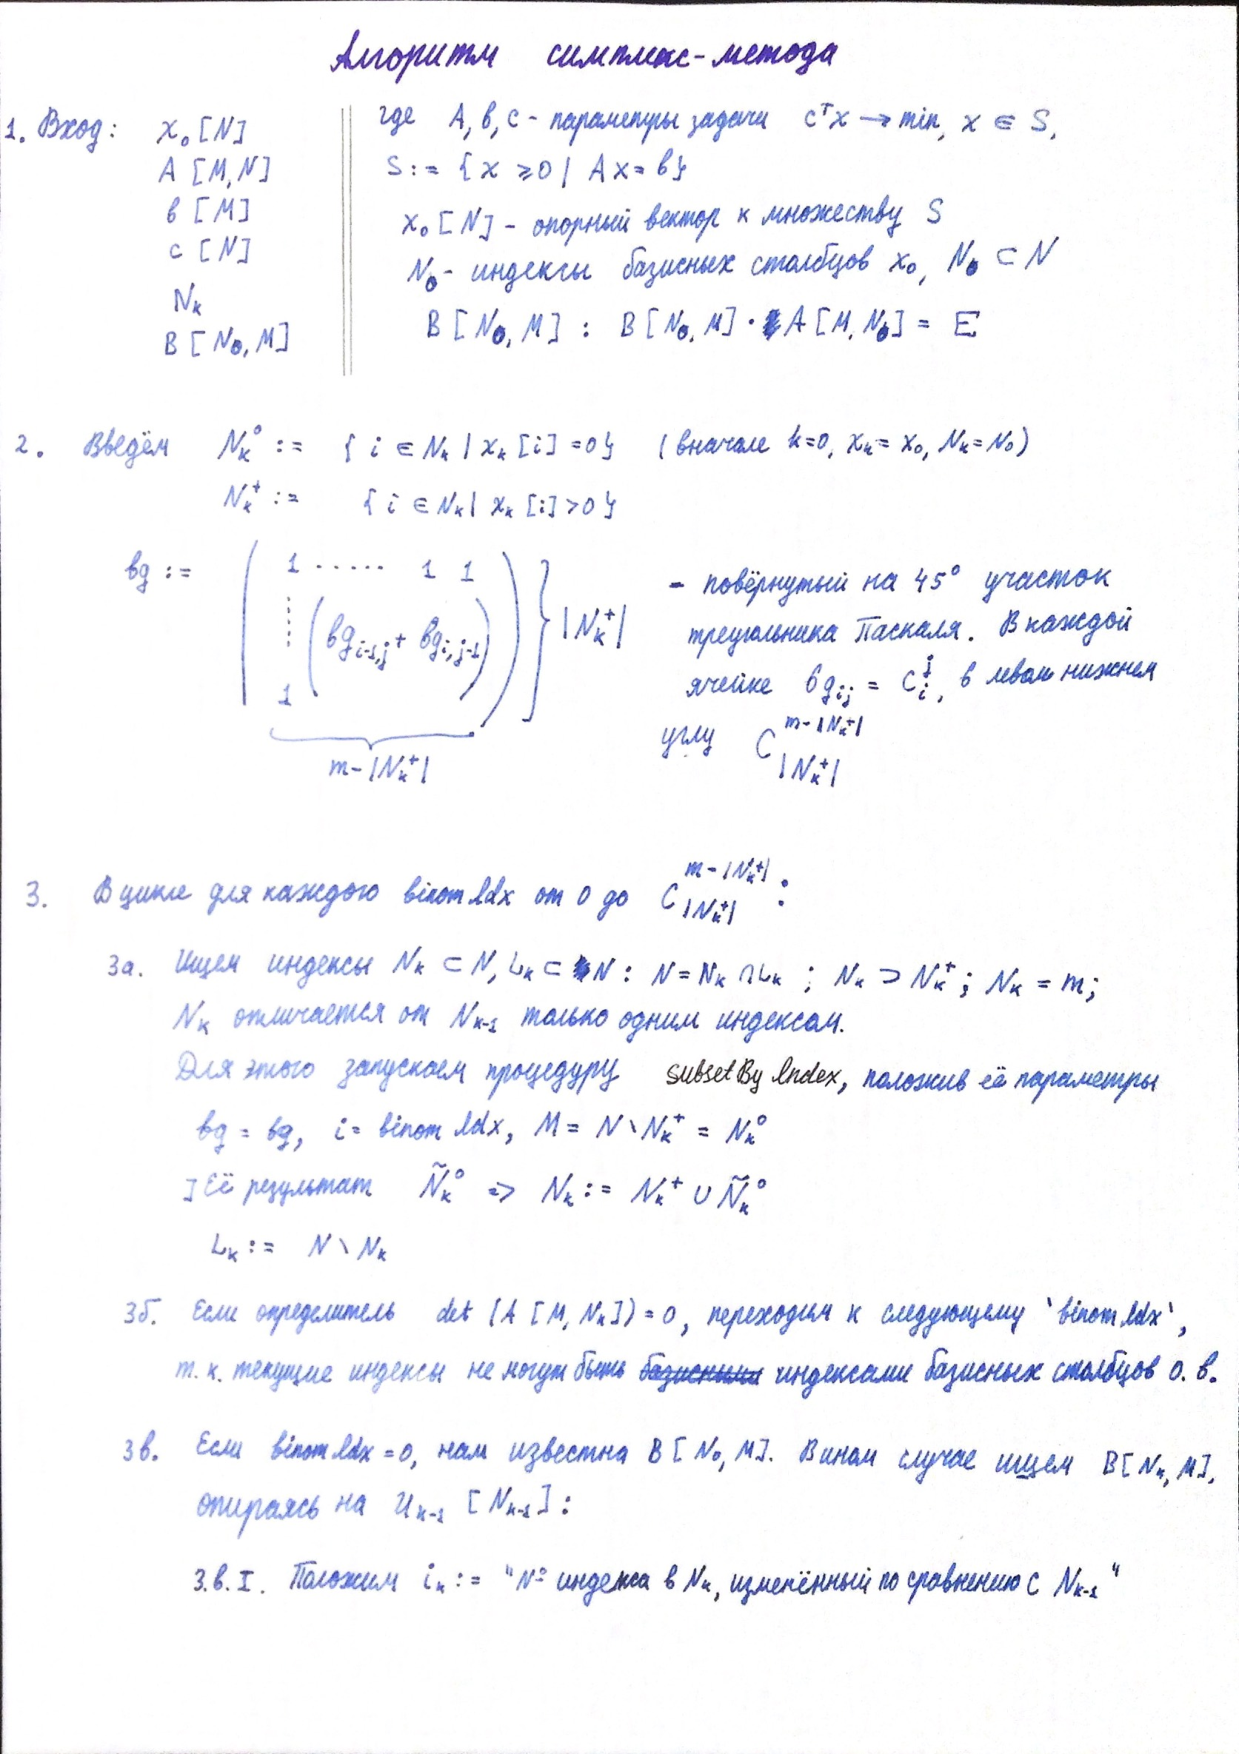
\includepdf[pages=-]{simplexEtcWritten.pdf}
\section{Результаты решения задачи}
\section{Оценка достоверности полученного результата}

\end{document}